\chapter[Password Selection and the Decoy Effect]{Password Selection and the Decoy Effect}\label{chap:decoy}

% Motivation
% users use weak passwords a
% users think l33t speak is more secure than other strategies (pasdjo finding)
% but this is not necessarily the case, passphrases might be a better alternative
% hard challenge: mental model of passphrases indicates users think they are too weak. 
% RQ: how can this be changed?
% RQ: reverse misconceptions with ``marketing'' \cite{Ashenden2013SecurityLikeSoap}
% RQ: in which way do suggestions influence self-selected passwords?



%TODO Result summary. 
\section{Background and Context}

Goal: influence / correct mental models of password strength, persuade users to consider alternative strategies. 

Criticism: this is unrealistic because memory interference effects prevent that this works for more than one account. -- yes, but for important accounts, this might still be worthwhile and people can more easily write down three words instead of an 8 character random sequence that might include ambiguous characters (0 and O); Kuo et al also say that writing down is a perfectly valid strategy \cite{Kuo2006HumanSelectionMnemonic}. (\todo{look up more researchers who argue in favor of writign down, e.g \cite{Kothari2017PasswordLogbooks} })

\paragraph{Suggestions}
Main topic: suggesting methods, feedback, modifications

\subsection{The Decoy Effect}
The decoy effect was discovered through research in consumer psychology. Buying a product often involves deciding between different alternatives. On a high level, products are easily comparable by their quality and price. These two dimensions build the foundation of the decoy effect. In one of the first experiments on ``asymmetric dominance'' effects, Huber \etal illustrate decision-making with a simple example to decide between different six-packs of beer\cite{Huber1982AsymetricallyDominated} (slightly adapted for simplicity): 
\begin{table}[!h]
\begin{tabular}{lrr}
	\textbf{Option} & \textbf{Price} & \textbf{Quality rating}\\
	(A) & \$4 & 50 /100\\
	(B) & \$6 & 70 /100\\
\end{tabular}
\end{table}

While option (A) is cheaper, it is also lower in quality. Spending \$2 more, the buyer will get a higher-quality beer (B). Buyers may have a preference for either lower price, or higher quality. Imagine the vendor wants to sell more of (A) because margins are higher for that product. To achieve this, Huber \etal explored adding a third option:
\begin{table}[!h]
\begin{tabular}{lrr}
	\textbf{Option} & \textbf{Price} & \textbf{Quality rating}\\
	(A) & \$4 & 50 /100 \\
	(B) & \$6 & 70 /100\\
	(C) & \$4 & 40 /100 \\
\end{tabular} 

\end{table}
Product (C) is as expensive as (A), but falls back in quality. Thus, buyers will get ``a better deal'' if they choose option (A) by comparison with (C). Options (B) and (C) are more difficult to compare, because both dimensions (price and quality) are higher in (B). Option (C) is thus called the \textit{decoy} that is \textit{dominated} by option (A) (\textit{target}) but not by option (B) (\textit{competitor}). 

- terminology: competitor, target, decoy.
- target is the item that we are trying to ``sell'' 
- competitor, as the name suggests, is a competing, but slightly less favorable sell for the vendor
- decoy: vendor does not intend to sell this, it acts as an unfavorable alternative that can be used as reference point / comparison.\\	

\begin{figure}
	\begin{subfigure}[t]{0.49\textwidth}
		\includegraphics[width=\textwidth]{figures/decoy/decoy-dimensions-general}
		\caption{Decoy placement options \cite{Huber1982AsymetricallyDominated}}
	\end{subfigure}
	\begin{subfigure}[t]{0.49\textwidth}
		\includegraphics[width=\textwidth]{figures/decoy/decoy-dimensions-beer}
		\caption{Example choice architecture for sixpack of beers.}
	\end{subfigure}
	\caption{\label{fig:decoy:general-construction} 
		General choice architecture overview to generate asymmetric dominance. 
		C = competitor, T = Target. The decoy can be placed at different positions in the spectrum, but needs to be dominated by the target (gray areay). Placement strategies for the decoy to increase the target's dominance: R = Range, R* = extreme range, F = frequency, RF = range and frequency.
	} 
\end{figure}

- broader concept: framing, salience, anchoring. 
- making choices, given a set of alternatives
- using a decoy choice architecture to influence the preferred option 

- terminology: competitor, target, decoy.
- target is the item that we are trying to ``sell'' 
- competitor, as the name suggests, is a competing, but slightly less favorable sell for the vendor
- decoy: vendor does not intend to sell this, it acts as an unfavorable alternative that can be used as reference point / comparison.

\subsubsection{Examples: Decoy Effects in UIs}


\subsection{Choice Architecture in Security and Privacy}
% make sure not to be too redundant. 

\section{Designing Decoy Options}
% Briefly point to first exploration report to mention a design that failed. 
General strategy (create logistic regression).

\section{Quantitative Evaluation}
\subsection{Methods}
no CS students: just like in \cite{Wash2016UnderstandingPasswordChoices}

live deployment. 

\subsection{Survey Results}
Mostly focus on the contents of the paper here

\subsection{Live-Deployment Data}
Talk about a couple of findings of the Roskilde dataset. 

\subsection{Limitations}


\section{Discussion}

\subsection{The Ineffectiveness of the Decoy Effect}


\subsection{Creativity Support}
As we have seen in chapter \ref{chap:pasdjo}, users know fairly well what makes a strong password. Thus, we can explain the stronger influence of the passphrase in several ways. There might be a gap between password strength perception and selection that is due to \textit{creativity}. It might be easier for people to decide upon a stronger password if they actually see it. This, however, will not work, if the password is absolutely unrelated to the person because this increases memorization efforts. 

Creativity is usually associated with the ``Openness'' personality trait (see chapter \ref{chap:pws_and_personality}). So we can suspect that people who show less of this trait might be more susceptible to a password suggestion. 

mental model influenced? -- look at qualitative data. 


\begin{figure}
	\centering
	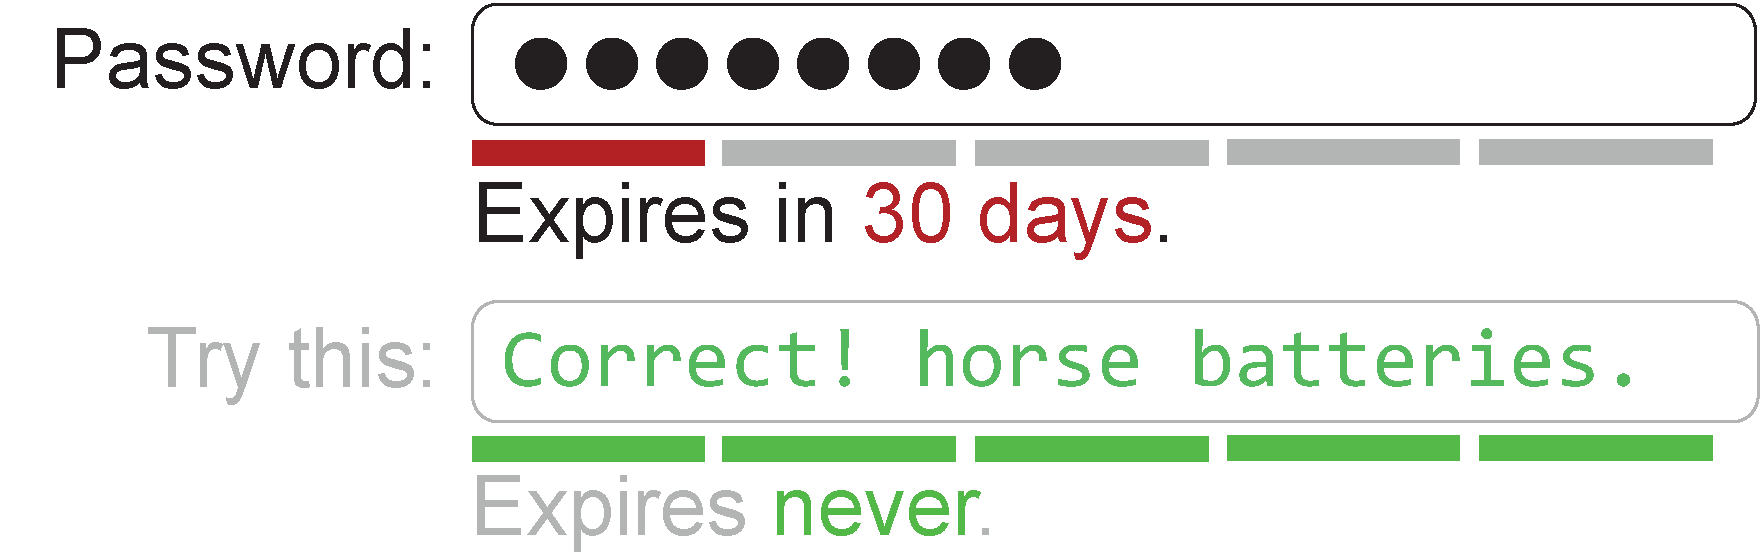
\includegraphics[width=0.7\linewidth]{figures/decoy/expire_mockup}
	\caption{\label{fig:decoy:expiremockup}Suggestion accompanied by enforced password expiration information.}
\end{figure}


\subsection{Application Areas}
it is not feasible to make users pick strong passwords for all accounts.
they already keep a list of ``important'' accounts that they wish to protect well, but stay in charge, so picking a strong memorable password for this type of account is vital to them. 

also, master passwords as gate-keeper to a larger number of passwords. 

\subsection{Personas}
which personas might be most most receptive to suggestions?

\section{Take-Aways}



